\documentclass{ximera}

%\usepackage{todonotes}

\newcommand{\todo}{}

\usepackage{esint} % for \oiint
\ifxake%%https://math.meta.stackexchange.com/questions/9973/how-do-you-render-a-closed-surface-double-integral
\renewcommand{\oiint}{{\large\bigcirc}\kern-1.56em\iint}
\fi


\graphicspath{
  {./}
  {ximeraTutorial/}
  {basicPhilosophy/}
  {functionsOfSeveralVariables/}
  {normalVectors/}
  {lagrangeMultipliers/}
  {vectorFields/}
  {greensTheorem/}
  {shapeOfThingsToCome/}
  {dotProducts/}
  {partialDerivativesAndTheGradientVector/}
  {../productAndQuotientRules/exercises/}
  {../normalVectors/exercisesParametricPlots/}
  {../continuityOfFunctionsOfSeveralVariables/exercises/}
  {../partialDerivativesAndTheGradientVector/exercises/}
  {../directionalDerivativeAndChainRule/exercises/}
  {../commonCoordinates/exercisesCylindricalCoordinates/}
  {../commonCoordinates/exercisesSphericalCoordinates/}
  {../greensTheorem/exercisesCurlAndLineIntegrals/}
  {../greensTheorem/exercisesDivergenceAndLineIntegrals/}
  {../shapeOfThingsToCome/exercisesDivergenceTheorem/}
  {../greensTheorem/}
  {../shapeOfThingsToCome/}
  {../separableDifferentialEquations/exercises/}
  {vectorFields/}
}

\newcommand{\mooculus}{\textsf{\textbf{MOOC}\textnormal{\textsf{ULUS}}}}

\usepackage{tkz-euclide}
\usepackage{tikz}
\usepackage{tikz-cd}
\usetikzlibrary{arrows}
\tikzset{>=stealth,commutative diagrams/.cd,
  arrow style=tikz,diagrams={>=stealth}} %% cool arrow head
\tikzset{shorten <>/.style={ shorten >=#1, shorten <=#1 } } %% allows shorter vectors

\usetikzlibrary{backgrounds} %% for boxes around graphs
\usetikzlibrary{shapes,positioning}  %% Clouds and stars
\usetikzlibrary{matrix} %% for matrix
\usepgfplotslibrary{polar} %% for polar plots
\usepgfplotslibrary{fillbetween} %% to shade area between curves in TikZ
%\usetkzobj{all}
\usepackage[makeroom]{cancel} %% for strike outs
%\usepackage{mathtools} %% for pretty underbrace % Breaks Ximera
%\usepackage{multicol}
\usepackage{pgffor} %% required for integral for loops



%% http://tex.stackexchange.com/questions/66490/drawing-a-tikz-arc-specifying-the-center
%% Draws beach ball
\tikzset{pics/carc/.style args={#1:#2:#3}{code={\draw[pic actions] (#1:#3) arc(#1:#2:#3);}}}



\usepackage{array}
\setlength{\extrarowheight}{+.1cm}
\newdimen\digitwidth
\settowidth\digitwidth{9}
\def\divrule#1#2{
\noalign{\moveright#1\digitwidth
\vbox{\hrule width#2\digitwidth}}}




% \newcommand{\RR}{\mathbb R}
% \newcommand{\R}{\mathbb R}
% \newcommand{\N}{\mathbb N}
% \newcommand{\Z}{\mathbb Z}

\newcommand{\sagemath}{\textsf{SageMath}}


%\renewcommand{\d}{\,d\!}
%\renewcommand{\d}{\mathop{}\!d}
%\newcommand{\dd}[2][]{\frac{\d #1}{\d #2}}
%\newcommand{\pp}[2][]{\frac{\partial #1}{\partial #2}}
% \renewcommand{\l}{\ell}
%\newcommand{\ddx}{\frac{d}{\d x}}

% \newcommand{\zeroOverZero}{\ensuremath{\boldsymbol{\tfrac{0}{0}}}}
%\newcommand{\inftyOverInfty}{\ensuremath{\boldsymbol{\tfrac{\infty}{\infty}}}}
%\newcommand{\zeroOverInfty}{\ensuremath{\boldsymbol{\tfrac{0}{\infty}}}}
%\newcommand{\zeroTimesInfty}{\ensuremath{\small\boldsymbol{0\cdot \infty}}}
%\newcommand{\inftyMinusInfty}{\ensuremath{\small\boldsymbol{\infty - \infty}}}
%\newcommand{\oneToInfty}{\ensuremath{\boldsymbol{1^\infty}}}
%\newcommand{\zeroToZero}{\ensuremath{\boldsymbol{0^0}}}
%\newcommand{\inftyToZero}{\ensuremath{\boldsymbol{\infty^0}}}



% \newcommand{\numOverZero}{\ensuremath{\boldsymbol{\tfrac{\#}{0}}}}
% \newcommand{\dfn}{\textbf}
% \newcommand{\unit}{\,\mathrm}
% \newcommand{\unit}{\mathop{}\!\mathrm}
% \newcommand{\eval}[1]{\bigg[ #1 \bigg]}
% \newcommand{\seq}[1]{\left( #1 \right)}
% \renewcommand{\epsilon}{\varepsilon}
% \renewcommand{\phi}{\varphi}


% \renewcommand{\iff}{\Leftrightarrow}

% \DeclareMathOperator{\arccot}{arccot}
% \DeclareMathOperator{\arcsec}{arcsec}
% \DeclareMathOperator{\arccsc}{arccsc}
% \DeclareMathOperator{\si}{Si}
% \DeclareMathOperator{\scal}{scal}
% \DeclareMathOperator{\sign}{sign}


%% \newcommand{\tightoverset}[2]{% for arrow vec
%%   \mathop{#2}\limits^{\vbox to -.5ex{\kern-0.75ex\hbox{$#1$}\vss}}}
% \newcommand{\arrowvec}[1]{{\overset{\rightharpoonup}{#1}}}
% \renewcommand{\vec}[1]{\arrowvec{\mathbf{#1}}}
% \renewcommand{\vec}[1]{{\overset{\boldsymbol{\rightharpoonup}}{\mathbf{#1}}}}

% \newcommand{\point}[1]{\left(#1\right)} %this allows \vector{ to be changed to \vector{ with a quick find and replace
% \newcommand{\pt}[1]{\mathbf{#1}} %this allows \vec{ to be changed to \vec{ with a quick find and replace
% \newcommand{\Lim}[2]{\lim_{\point{#1} \to \point{#2}}} %Bart, I changed this to point since I want to use it.  It runs through both of the exercise and exerciseE files in limits section, which is why it was in each document to start with.

% \DeclareMathOperator{\proj}{\mathbf{proj}}
% \newcommand{\veci}{{\boldsymbol{\hat{\imath}}}}
% \newcommand{\vecj}{{\boldsymbol{\hat{\jmath}}}}
% \newcommand{\veck}{{\boldsymbol{\hat{k}}}}
% \newcommand{\vecl}{\vec{\boldsymbol{\l}}}
% \newcommand{\uvec}[1]{\mathbf{\hat{#1}}}
% \newcommand{\utan}{\mathbf{\hat{t}}}
% \newcommand{\unormal}{\mathbf{\hat{n}}}
% \newcommand{\ubinormal}{\mathbf{\hat{b}}}

% \newcommand{\dotp}{\bullet}
% \newcommand{\cross}{\boldsymbol\times}
% \newcommand{\grad}{\boldsymbol\nabla}
% \newcommand{\divergence}{\grad\dotp}
% \newcommand{\curl}{\grad\cross}
%\DeclareMathOperator{\divergence}{divergence}
%\DeclareMathOperator{\curl}[1]{\grad\cross #1}
% \newcommand{\lto}{\mathop{\longrightarrow\,}\limits}

% \renewcommand{\bar}{\overline}

\colorlet{textColor}{black}
\colorlet{background}{white}
\colorlet{penColor}{blue!50!black} % Color of a curve in a plot
\colorlet{penColor2}{red!50!black}% Color of a curve in a plot
\colorlet{penColor3}{red!50!blue} % Color of a curve in a plot
\colorlet{penColor4}{green!50!black} % Color of a curve in a plot
\colorlet{penColor5}{orange!80!black} % Color of a curve in a plot
\colorlet{penColor6}{yellow!70!black} % Color of a curve in a plot
\colorlet{fill1}{penColor!20} % Color of fill in a plot
\colorlet{fill2}{penColor2!20} % Color of fill in a plot
\colorlet{fillp}{fill1} % Color of positive area
\colorlet{filln}{penColor2!20} % Color of negative area
\colorlet{fill3}{penColor3!20} % Fill
\colorlet{fill4}{penColor4!20} % Fill
\colorlet{fill5}{penColor5!20} % Fill
\colorlet{gridColor}{gray!50} % Color of grid in a plot

\newcommand{\surfaceColor}{violet}
\newcommand{\surfaceColorTwo}{redyellow}
\newcommand{\sliceColor}{greenyellow}




\pgfmathdeclarefunction{gauss}{2}{% gives gaussian
  \pgfmathparse{1/(#2*sqrt(2*pi))*exp(-((x-#1)^2)/(2*#2^2))}%
}


%%%%%%%%%%%%%
%% Vectors
%%%%%%%%%%%%%

%% Simple horiz vectors
\renewcommand{\vector}[1]{\left\langle #1\right\rangle}


%% %% Complex Horiz Vectors with angle brackets
%% \makeatletter
%% \renewcommand{\vector}[2][ , ]{\left\langle%
%%   \def\nextitem{\def\nextitem{#1}}%
%%   \@for \el:=#2\do{\nextitem\el}\right\rangle%
%% }
%% \makeatother

%% %% Vertical Vectors
%% \def\vector#1{\begin{bmatrix}\vecListA#1,,\end{bmatrix}}
%% \def\vecListA#1,{\if,#1,\else #1\cr \expandafter \vecListA \fi}

%%%%%%%%%%%%%
%% End of vectors
%%%%%%%%%%%%%

%\newcommand{\fullwidth}{}
%\newcommand{\normalwidth}{}



%% makes a snazzy t-chart for evaluating functions
%\newenvironment{tchart}{\rowcolors{2}{}{background!90!textColor}\array}{\endarray}

%%This is to help with formatting on future title pages.
\newenvironment{sectionOutcomes}{}{}



%% Flowchart stuff
%\tikzstyle{startstop} = [rectangle, rounded corners, minimum width=3cm, minimum height=1cm,text centered, draw=black]
%\tikzstyle{question} = [rectangle, minimum width=3cm, minimum height=1cm, text centered, draw=black]
%\tikzstyle{decision} = [trapezium, trapezium left angle=70, trapezium right angle=110, minimum width=3cm, minimum height=1cm, text centered, draw=black]
%\tikzstyle{question} = [rectangle, rounded corners, minimum width=3cm, minimum height=1cm,text centered, draw=black]
%\tikzstyle{process} = [rectangle, minimum width=3cm, minimum height=1cm, text centered, draw=black]
%\tikzstyle{decision} = [trapezium, trapezium left angle=70, trapezium right angle=110, minimum width=3cm, minimum height=1cm, text centered, draw=black]


\title{Shifting Domain}

\begin{document}

\begin{abstract}
same characteristics
\end{abstract}
\maketitle








One way to create a new function from an existing function is to shift all of the domain numbers in the function pairs. \\

\[
(a, b) \mapsto (a + k, b)
\]



\textbf{\textcolor{blue!55!black}{$\blacktriangleright$}} How do we describe a shifting domain? \\

We want a graphical description. We want an algebraic description. \\




Below is the piecewise-defined function, $T(v)$.  The variable $v$ is representing the domain values from the set $(-4,-1] \cup [1,7)$.




\[
T(v) = 
\begin{cases}
  2v-1 & \text{ if }  -4 < v \leq -1 \\
  -v+3 & \text{ if } 1 \leq v < 7
\end{cases}
\]


On the interval $(-4, -1]$, the graph is a line segment for $T(v) = 2v-1$, a linear function with a restricted domain. \\



On the interval $[1, 7)$, the graph is another line segment for $T(v) = -v+3$, a linear function with a restricted domain. \\




Graph of $y = T(v)$.
\begin{image}
\begin{tikzpicture}
	\begin{axis}[
            domain=-10:10, ymax=10, xmax=10, ymin=-10, xmin=-10,
            axis lines =center, xlabel=$v$, ylabel=${y=T(v)}$, 
            ytick={-10,-8,-6,-4,-2,2,4,6,8,10},
            xtick={-10,-8,-6,-4,-2,2,4,6,8,10},
            ticklabel style={font=\scriptsize},
            every axis y label/.style={at=(current axis.above origin),anchor=south},
            every axis x label/.style={at=(current axis.right of origin),anchor=west},
            axis on top
          ]
          
	\addplot [draw=penColor,very thick,smooth,domain=(-4:-1)] {2*x-1};
	\addplot [draw=penColor,very thick,smooth,domain=(1:7)] {-x+3};
	\addplot[color=penColor,only marks,mark=*] coordinates{(-1,-3)}; 
	\addplot[color=penColor,fill=white,only marks,mark=*] coordinates{(-4,-9)}; 
	\addplot[color=penColor,only marks,mark=*] coordinates{(1,2)}; 
	\addplot[color=penColor,fill=white,only marks,mark=*] coordinates{(7,-4)}; 


    \end{axis}
\end{tikzpicture}
\end{image}







The domain of $T$ has two maximal intervals:, $(-4,-1]$ and $[1,7)$.  These correspond to two line segments on the graph. The endpoints give us four strategic points on the graph: 

\begin{itemize}

\item $(-4, -9)$, which is an open dot on the graph.
\item $(-1, -3)$, which is a closed dot on the graph.
\item $(1, 2)$, which is a closed dot on the graph.
\item $(7, -4)$, which is an open dot on the graph.

\end{itemize}




\subsection*{A New Function}

$B(k)$ is a new function we are creating, but its definition is based on $T(v)$.


\textbf{\textcolor{blue!55!black}{$\blacktriangleright$ Define $B$ by $B(k) = T(k+3)$ with the induced domain.}} 



\textbf{Questions:} 
\begin{itemize}
  \item What is the domain of $B$?
  \item What are the corresponding strategic points on the graph of $B$?
  \item What is the formula for $B$?
\end{itemize}



\textbf{\textcolor{purple!85!blue}{First Question:}}   What is the domain of $B$?


\begin{explanation}

In $B(k)$, $k$ is representing the values of the domain of $B$. \\
In $T(k + 3)$,  $k+3$ is now representing the domain values of $T$.  \\
Therefore $k+3$ must take on the values in $(-4,-1] \cup [1,7)$.

\[     k+3 \in      (-4,-1] \cup [1,7)     \]


$k$ must be in a similar set, but shifted to the left by $3$, because we need to subtract $3$ from $k+3$ to get $k$.


\[     k \in      \left( -7,\answer{-4} \right] \cup \left[ \answer{-2},4 \right)     \]


The domain of $B$ is $(-7,-4] \cup [-2,4)$.   \\

It was ``induced'' from the domain of $T$ through the definition of $B$, which is using $T$.  The values in the domain of $B$ are real numbers, $k$, such that $k+3$ is in the domain of $T$.

The domain has shifted. 


But, the structure of the function hasn't changed.  The same formulas are in use.  They are just used by different domain numbers.



\end{explanation}




\textbf{\textcolor{purple!85!blue}{Second Question:}}  The graph of $T$ had four strategic points.  What are the corresponding points on the graph of $B$?


We have four strategic points on the graph of $T$: 

\begin{itemize}

\item $(-4, -9)$, which is an open dot on the graph of $T$.
\item $(-1, -3)$, which is a closed dot on the graph of $T$.
\item $(1, 2)$, which is a closed dot on the graph of $T$.
\item $(7, -4)$, which is an open dot on the graph of $T$.

\end{itemize}


How do these translate to strategic points on the graph of $B$?


\begin{itemize}

\item $(-4, -9)$ tells us that $T(-4) = -9$.   
To match the template $B(k) = T(k+3)$, we need $k=-7$.  Replacing $k$ with $-7$ gives us
\[ B(-7) = T(-7 + 3) = T(-4) = -9\]
$B(-7) = -9$ and the point $(-7, -9)$ is on the graph of $B$. It is an open dot. \\


\item $(-1, -3)$ tells us that $T(-1) = -3$.   
To match the template $B(k) = T(k+3)$, we need $k=-4$.  Replacing $k$ with $-4$ gives us
\[ B(-4) = T(-4 + 3) = T(-1) = -3\]
$B(-4) = -3$ and the point $(-4, -3)$ is on the graph of $B$. It is a closed dot. \\


\item $(1, 2)$ tells us that $T(1) = 2$.   
To match the template $B(k) = T(k+3)$, we need $k=-2$.  Replacing $k$ with $-2$ gives us
\[ B(-2) = T(-2 + 3) = T(1) = 2\]
$B(-2) = 2$ and the point $(-2, 2)$ is on the graph of $B$. It is a closed dot. \\


\item $(7, -4)$ tells us that $T(7) = -4$.   
To match the template $B(k) = T(k+3)$, we need $k=4$.  Replacing $k$ with $4$ gives us
\[ B(4) = T(4 + 3) = T(7) = -4\]
$B(4) = -4$ and the point $(4, -4)$ is on the graph of $B$. It is an open dot.


\end{itemize}














\textbf{\textcolor{purple!85!blue}{Third Question:}} What is the formula for $B$?



\begin{explanation}
When $k \in (-7,-4]$, then $k+3 \in \left(\answer{-4},\answer{-1}\right]$.  

$v=k+3$, so $v \in \left(\answer{-4},\answer{-1}\right]$ and we are using the formula $2v-1$ with $v=k+3$. 

All together: when $k \in (-7,-4]$, then $B(k) = 2(k+3)-1$.
\end{explanation}



\begin{explanation}
When $k \in [-2,4)$, then $k+3 \in \left[\answer{1},\answer{7}\right)$.  

$v=k+3$, so $v \in \left[\answer{1},\answer{7}\right)$ and we are using the formula $-v+3$ with $v=k+3$.

All together: when $k \in [-2,4)$, then $B(k) = -(k+3)+3$.
\end{explanation}












\[
B(k) = 
\begin{cases}
  2k+5 & \text{ if }  -7 < k \leq -4 \\
  -k & \text{ if } -2 \leq k < 4
\end{cases}
\]





Graph of $z = B(k)$.

\begin{image}
\begin{tikzpicture}
	\begin{axis}[
            domain=-10:10, ymax=10, xmax=10, ymin=-10, xmin=-10,
            axis lines =center, xlabel=$k$, ylabel=${z=B(k)}$,
            ytick={-10,-8,-6,-4,-2,2,4,6,8,10},
            xtick={-10,-8,-6,-4,-2,2,4,6,8,10},
            ticklabel style={font=\scriptsize},
            every axis y label/.style={at=(current axis.above origin),anchor=south},
            every axis x label/.style={at=(current axis.right of origin),anchor=west},
            axis on top
          ]
          
	\addplot [draw=penColor,very thick,smooth,domain=(-7:-4)] {2*x+5};
	\addplot [draw=penColor,very thick,smooth,domain=(-2:4)] {-x};
	\addplot[color=penColor,only marks,mark=*] coordinates{(-4,-3)}; 
	\addplot[color=penColor,fill=white,only marks,mark=*] coordinates{(-7,-9)}; 
	\addplot[color=penColor,only marks,mark=*] coordinates{(-2,2)}; 
	\addplot[color=penColor,fill=white,only marks,mark=*] coordinates{(4,-4)}; 


    \end{axis}
\end{tikzpicture}
\end{image}






When we look at the graphs side-by-side, we can see that the graph of $T$ has simply shifted left $3$ to become the graph of $B$.








\begin{image}
\begin{tikzpicture}
	\begin{axis}[name = leftgraph,
            domain=-10:10, ymax=10, xmax=10, ymin=-10, xmin=-10,
            axis lines =center, xlabel=$v$, ylabel={$y=T(v)$},
            every axis y label/.style={at=(current axis.above origin),anchor=south},
            every axis x label/.style={at=(current axis.right of origin),anchor=west},
            axis on top
          ]
          
	\addplot [draw=penColor,very thick,smooth,domain=(-4:-1)] {2*x-1};
	\addplot [draw=penColor,very thick,smooth,domain=(1:7)] {-x+3};
	\addplot[color=penColor,only marks,mark=*] coordinates{(-1,-3)}; 
	\addplot[color=penColor,fill=white,only marks,mark=*] coordinates{(-4,-9)}; 
	\addplot[color=penColor,only marks,mark=*] coordinates{(1,2)}; 
	\addplot[color=penColor,fill=white,only marks,mark=*] coordinates{(7,-4)}; 


    \end{axis}
	\begin{axis}[at={(leftgraph.outer east)},anchor=outer west, 
            domain=-10:10, ymax=10, xmax=10, ymin=-10, xmin=-10,
            axis lines =center, xlabel=$k$, ylabel={$z=B(k)$},
            every axis y label/.style={at=(current axis.above origin),anchor=south},
            every axis x label/.style={at=(current axis.right of origin),anchor=west},
            axis on top
          ]
          
	\addplot [draw=penColor,very thick,smooth,domain=(-7:-4)] {2*x+5};
	\addplot [draw=penColor,very thick,smooth,domain=(-2:4)] {-x};
	\addplot[color=penColor,only marks,mark=*] coordinates{(-4,-3)}; 
	\addplot[color=penColor,fill=white,only marks,mark=*] coordinates{(-7,-9)}; 
	\addplot[color=penColor,only marks,mark=*] coordinates{(-2,2)}; 
	\addplot[color=penColor,fill=white,only marks,mark=*] coordinates{(4,-4)}; 


    \end{axis}


\end{tikzpicture}
\end{image}
The structure of the two graphs hasn't changed. \\



From the definition, $B(k) = T(k+3)$, we can see that $v=k+3$, or $k=v-3$.  All of the $k$-values are $3$ less than the $v$-values.  $B$ is $T$ shifted left $3$.





\begin{warning} \textbf{\textcolor{red!80!black}{Variables}} \\

Notice that four different variables, $v$, $y$, $k$, and $z$, are used to describe the domain and range values of $T$ and $B$.  We are using separate names for the different types of values to keep everything clear. If we use the same variable to represent both domains, then we run into problems.




\textcolor{blue!55!black}{
\textbf{For instance...} Suppose we use $x$ to represent values in both domains.  Then $x = 0$ is a possibility for $B$.  $B(0) = 0$.  However, if we write $x = 0$ and $x$ is also representing the domain of $T$, then we are implying that $T(0)$ is a valid number.  However, $0$ is not in the domain of $T$.
}


We use variables to help us think about structure and relationships.  For this reason, we should not use the same variable to represent values from two different sets in the same situation.


Similarly, the two vertical axes have been labelled $y$ and $z$.  If we use $y$ to represent both axes, then we are using $y$ to represent both ranges and that also leads to communication problems.

We will avoid using the same variables or labels for values from different sets.

\end{warning}

























\begin{example} Shifting the Domain 






\[
V(h) = 
\begin{cases}
  -2h-3 & \text{ on } [-6, -2]   \\
  -(h+3)(h-3) & \text{ on } (-2, 4]  \\
  \frac{7h}{4} - 8 & \text{ on } (4,6)
\end{cases}
\]



A graph always helps our thinking. Here is the graph of $y = V(h)$.








\begin{image}
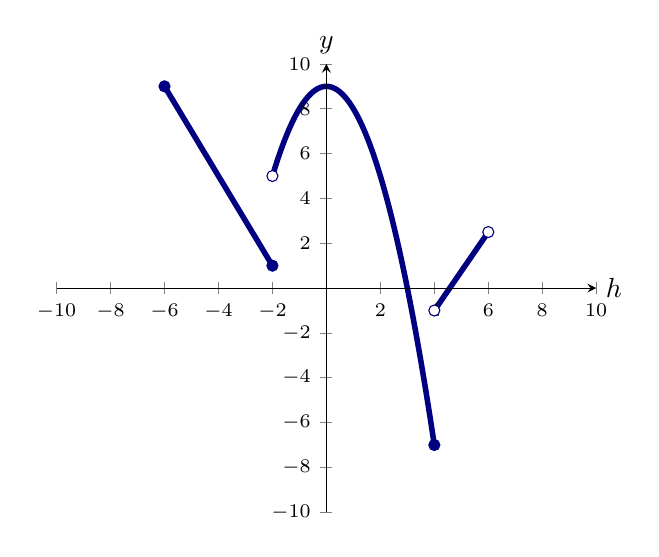
\begin{tikzpicture} 
  \begin{axis}[
            domain=-10:10, ymax=10, xmax=10, ymin=-10, xmin=-10,
            axis lines =center, xlabel=$h$, ylabel=$y$,
            ytick={-10,-8,-6,-4,-2,2,4,6,8,10},
            xtick={-10,-8,-6,-4,-2,2,4,6,8,10},
            ticklabel style={font=\scriptsize},
            every axis y label/.style={at=(current axis.above origin),anchor=south},
            every axis x label/.style={at=(current axis.right of origin),anchor=west},
            axis on top
          ]
          
      \addplot [line width=2, penColor, smooth,samples=100,domain=(-6:-2)] {-2*x-3};
          \addplot [line width=2, penColor, smooth,samples=100,domain=(-2:4)] {-1*(x+3)*(x-3))};
          \addplot [line width=2, penColor, smooth,samples=100,domain=(4:6)] {1.75*x-8};




      \addplot[color=penColor,fill=penColor,only marks,mark=*] coordinates{(-6,9)};
      \addplot[color=penColor,fill=penColor,only marks,mark=*] coordinates{(-2,1)};

      \addplot[color=penColor,fill=white,only marks,mark=*] coordinates{(-2,5)};
      \addplot[color=penColor,fill=penColor,only marks,mark=*] coordinates{(4,-7)};

      \addplot[color=penColor,fill=white,only marks,mark=*] coordinates{(4,-1)};
      \addplot[color=penColor,fill=white,only marks,mark=*] coordinates{(6,2.5)};


           

  \end{axis}
\end{tikzpicture}
\end{image}





Define a new function by $f(x) = V(x-1)$ with the induced domain.

The domain of $V$ is $[-6, 6)$.  These values are represented by $x-1$ in this definition, because $x-1$ is the expression inside the parentheses for $V$ and that is where the expression lives for the domain values of $V$.

$x$ represents the domain values of $f$.   If $x - 1 \in [-6, 6)$, then $x \in \left[\answer{-5}, \answer{7}\right)$.  This is the domain for $f$.  It is shifted $1$ to the right from the domain of $V$.  The individual maximal intervals become $[-5, -1]$, $\left(\answer{-1}, \answer{5}\right]$, and $[5, 7)$.





\[
f(x) = V(x-1) = 
\begin{cases}
  -2(x-1)-3 & \text{ on } [-5, -1]   \\
  -((x-1)+3)((x-1)-3) & \text{ on } (-1, 5]  \\
  \frac{7(x-1)}{4} - 8 & \text{ on } (5, 7)
\end{cases}
\]





\[
f(x) = 
\begin{cases}
  -2x - 1 &  [-5, -1]   \\
  -(x+2)(x-4) &  (-1, 5]  \\
  \frac{7(x-1)}{4} - 8 &  (5, 7)
\end{cases}
\]

















\begin{image}
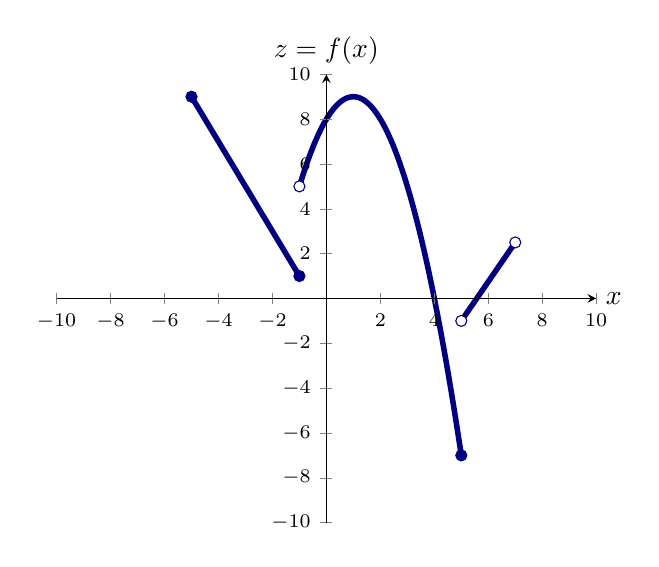
\begin{tikzpicture} 
  \begin{axis}[
            domain=-10:10, ymax=10, xmax=10, ymin=-10, xmin=-10,
            axis lines =center, xlabel=$x$, ylabel={$z=f(x)$},
            ytick={-10,-8,-6,-4,-2,2,4,6,8,10},
            xtick={-10,-8,-6,-4,-2,2,4,6,8,10},
            ticklabel style={font=\scriptsize},
            every axis y label/.style={at=(current axis.above origin),anchor=south},
            every axis x label/.style={at=(current axis.right of origin),anchor=west},
            axis on top
          ]
          
          \addplot [line width=2, penColor, smooth,samples=100,domain=(-5:-1)] {-2*x-1};
          \addplot [line width=2, penColor, smooth,samples=100,domain=(-1:5)] {-1*(x+2)*(x-4))};
          \addplot [line width=2, penColor, smooth,samples=100,domain=(5:7)] {1.75*(x-1)-8};




      \addplot[color=penColor,fill=penColor,only marks,mark=*] coordinates{(-5,9)};
      \addplot[color=penColor,fill=penColor,only marks,mark=*] coordinates{(-1,1)};

      \addplot[color=penColor,fill=white,only marks,mark=*] coordinates{(-1,5)};
      \addplot[color=penColor,fill=penColor,only marks,mark=*] coordinates{(5,-7)};

      \addplot[color=penColor,fill=white,only marks,mark=*] coordinates{(5,-1)};
      \addplot[color=penColor,fill=white,only marks,mark=*] coordinates{(7,2.5)};


           

  \end{axis}
\end{tikzpicture}
\end{image}




The graph has the same three shapes. The corresponding endpoints are hollow or filled as they were in the graph of $y=V(h)$.



\end{example}
















\begin{example} Shifting Domain


Let $P(t)$ be a function with domain $[-11, -7) \cup \{ -6 \} \cup [-4,3) \cup (4, 7] \cup \{ 8 \} \cup [9, 10)$.

Let $g(w)$ be defined as a shifted domain version of $P(t)$.  The domain of $g(w)$ is $[-7, -3) \cup \{ -2 \} \cup [0,7) \cup (8, 11] \cup \{ 12 \} \cup [13, 14)$.

\begin{itemize}
\item In terms of $t$, $w = \answer{t+4}$ 
\item In terms of $w$, $t = \answer{w-4}$.  \\
\end{itemize}


\begin{itemize}
\item $g(w) = P\left(\answer{w-4}\right)$ \\

\item $P(t) = g\left(\answer{t+4}\right)$ \\
\end{itemize}

\end{example}














When a new function is defined by a domain shift of an existing function, then there are two different domains.  \\


It is natural to think, "\textbf{\textcolor{purple!85!blue}{What was done to the old domain to get the new one?}}"

Suppose $f(t)$ is an existing function with domain $[-3, 5]$.

Define a new function $g(x)$ as $g(x) = f(x-8)$ with the induced domain.



\begin{itemize}
\item ``$t$'' represents elements of the old domain of $f(t)$.  
\item ``$x$'' represents elements of the new domain of $g(x)$.  
\end{itemize}




It is natural to ask ``what happens to $t$ to get $x$?''  



\begin{center}
\textbf{\textcolor{red!70!black}{But that is NOT how it is presented to us.}}
\end{center}






We are told that $t=x-8$.  But that is what happens to $x$ to get $t$.  That is backwards of how we naturally think about old and new.  We need to solve for $x$ to see what is done to $t$.

\[ t+8=x \]

To get the new domain number, $x$, add $8$ to the old domain numbers $t$.  This tells us that the graph of $g$ will be shifted to the right by $8$, compared to the position of the graph of $f$.


It is reversed from how it was originally defined, $g(x) = f(x-8)$, because the ``inside'' of $f$ is $x-8$ here.  That is not what is done to $t$.  When we solve $t=x-8$ for $x$, we reverse all of the arithmetic and discover what was done to $t$.




\begin{example} Shifting Domain


Let $D(y)$ be a function with its domain.

Let $K(r)$ be defined as $K(r) = D(r+7)$ with its induced domain.


Then the domain of $K$ is the domain of $D$, but shifted \wordChoice{\choice[correct] {Left} \choice {Right}} by 
\wordChoice{\choice{5} \choice{6} \choice[correct]{7}}


Then the graph of $K$ is the graph of $D$, but shifted \wordChoice{\choice[correct] {Left} \choice {Right}} by 
\wordChoice{\choice{5} \choice{6} \choice[correct]{7}}




\end{example}












\begin{example} Shifting Domain


Let $f(w)$ be a function with its domain.

Let $g(t)$ be defined as $g(t) = f(t-3)$ with its induced domain.


Then the domain of $g$ is the domain of $f$, but shifted \wordChoice{\choice{Left} \choice [correct]{Right}} by 
\wordChoice{\choice{1} \choice{2} \choice[correct]{3}}


Then the graph of $g$ is the graph of $f$, but shifted \wordChoice{\choice{Left} \choice [correct]{Right}} by 
\wordChoice{\choice{1} \choice{2} \choice[correct]{3}}




\end{example}














































$\blacktriangleright$ Graphically, shifting the domain of a function appears to shift the graph horizontally - left or right.  The shape of the graph doesn't change.  The whole graph moves rigidly left or right.  All points move the same distance horizontally. \\


\begin{itemize}
\item Let $F(x)$ be a function with its domain.

\item Let $G(t)$ be a new function defined as $G(t) = F(t+d_0)$ with its induced domain, where $d_0$ is a fixed constant.
\end{itemize}



We begin with the function $F$.  The domain values of $F$ are represented by $x$.  We then define a new function, $G$. The domain values of $G$ are represented by $t$. 

$F$ and $G$ are connected.  To evaluate $G$ at $t$, you evaluate $F$ at $t + d_0$, where $d_0$ is some constant.  Therefore, $t + d_0$ are $x$-values. We have $x = t + d_0$.  This tells us what to do to $t$ to get $x$.  However, that is not how our story is told.  Our story begins with $F$ and then $G$ is defined from $F$.  

We want to know how to get $t$ from $x$.  


\begin{itemize}
\item $x = t + d_0$

\item $x - d_0 = t$
\end{itemize}


To get corresponding values of $t$ from values of $x$, subtract $d_0$.   



$\blacktriangleright$  The graph of $G$ is obtained from the graph of $F$ by subtracting $d_0$ from domain values of $F$, which appears to be reverse of the definition, $G(t) = F(t+d_0)$.  That is because the definition tells how to get the old domain for $F$, rather than getting the new domain for $G$.



\begin{example} Shifting Horizontally




Graph of $y = T(v)$.

\begin{image}
\begin{tikzpicture}
  \begin{axis}[
            domain=-10:10, ymax=10, xmax=10, ymin=-10, xmin=-10,
            axis lines =center, xlabel=$v$, ylabel=$y$,
            ytick={-10,-8,-6,-4,-2,2,4,6,8,10},
            xtick={-10,-8,-6,-4,-2,2,4,6,8,10},
            ticklabel style={font=\scriptsize},
            every axis y label/.style={at=(current axis.above origin),anchor=south},
            every axis x label/.style={at=(current axis.right of origin),anchor=west},
            axis on top
          ]
          
  \addplot [draw=penColor,very thick,smooth,domain=(-7:-4)] {-x-6};
  \addplot [draw=penColor,very thick,smooth,domain=(-2:1)] {-7};
  \addplot [draw=penColor,very thick,smooth,domain=(1:7)] {-x+7};
  
  \addplot[color=penColor,only marks,mark=*] coordinates{(-7,1)}; 
  \addplot[color=penColor,fill=white,only marks,mark=*] coordinates{(-4,-2)}; 
  \addplot[color=penColor,only marks,mark=*] coordinates{(-2,-7)}; 
  \addplot[color=penColor,only marks,mark=*] coordinates{(1,-7)}; 
  \addplot[color=penColor,only marks,mark=*] coordinates{(1,6)}; 
  \addplot[color=penColor,fill=white,only marks,mark=*] coordinates{(7,0)}; 


    \end{axis}
\end{tikzpicture}
\end{image}


Define a new function $W$ by $W(h)=T(h+3)$, with the induced domain.

Which graph below is the graph of $z=W(h)$?





\begin{image}
\begin{tikzpicture}
  \begin{axis}[name = leftgraph,
            domain=-10:10, ymax=10, xmax=10, ymin=-10, xmin=-10,
            axis lines =center, xlabel=$h$, ylabel=$z$,
            ytick={-10,-8,-6,-4,-2,2,4,6,8,10},
            xtick={-10,-8,-6,-4,-2,2,4,6,8,10},
            ticklabel style={font=\scriptsize},
            every axis y label/.style={at=(current axis.above origin),anchor=south},
            every axis x label/.style={at=(current axis.right of origin),anchor=west},
            axis on top
          ]
          
  \addplot [draw=penColor,very thick,smooth,domain=(-10:-7)] {-(x+3)-6};
  \addplot [draw=penColor,very thick,smooth,domain=(-5:-2)] {-7};
  \addplot [draw=penColor,very thick,smooth,domain=(-2:4)] {-(x+3)+7};
  
  \addplot[color=penColor,only marks,mark=*] coordinates{(-10,1)}; 
  \addplot[color=penColor,fill=white,only marks,mark=*] coordinates{(-7,-2)}; 
  \addplot[color=penColor,only marks,mark=*] coordinates{(-5,-7)}; 
  \addplot[color=penColor,only marks,mark=*] coordinates{(-2,-7)}; 
  \addplot[color=penColor,only marks,mark=*] coordinates{(-2,6)}; 
  \addplot[color=penColor,fill=white,only marks,mark=*] coordinates{(4,0)}; 


    \end{axis}
  \begin{axis}[at={(leftgraph.outer east)},anchor=outer west, 
            domain=-10:10, ymax=10, xmax=10, ymin=-10, xmin=-10,
            axis lines =center, xlabel=$h$, ylabel=$z$,
            ytick={-10,-8,-6,-4,-2,2,4,6,8,10},
            xtick={-10,-8,-6,-4,-2,2,4,6,8,10},
            ticklabel style={font=\scriptsize},
            every axis y label/.style={at=(current axis.above origin),anchor=south},
            every axis x label/.style={at=(current axis.right of origin),anchor=west},
            axis on top
          ]
          
  \addplot [draw=penColor,very thick,smooth,domain=(-4:-1)] {-(x-3)-6};
  \addplot [draw=penColor,very thick,smooth,domain=(1:4)] {-7};
  \addplot [draw=penColor,very thick,smooth,domain=(4:10)] {-(x-3)+7};
  
  \addplot[color=penColor,only marks,mark=*] coordinates{(-4,1)}; 
  \addplot[color=penColor,fill=white,only marks,mark=*] coordinates{(-1,-2)}; 
  \addplot[color=penColor,only marks,mark=*] coordinates{(1,-7)}; 
  \addplot[color=penColor,only marks,mark=*] coordinates{(4,-7)}; 
  \addplot[color=penColor,only marks,mark=*] coordinates{(4,6)}; 
  \addplot[color=penColor,fill=white,only marks,mark=*] coordinates{(10,0)}; 


    \end{axis}


\end{tikzpicture}
\end{image}





\begin{multipleChoice}
\choice[correct]{graph on the left}
\choice{graph on the right}
\end{multipleChoice}

To figure this out, we need to know how to get the new variable $h$ from the old variable $v$. \\




\begin{itemize}
\item $h$ represents the domain of $W$. 
\item $v$ represents the domain of $T$.  
\item $v$ = $h+3$
\end{itemize}


These tell us that $v-3 = h$ and the graph of $W$ is the graph of $T$ shifted left $3$.



\end{example}


The shape of the graph didn't change. It just slid to the left. There are still three pieces. \\




\begin{itemize}
\item The domain still has a gap of length $2$ in it.  
\item The middle piece is still horizontal.  
\item The solid and hollow endpoint dots are still in the same positions. 
\end{itemize}





Shifting doesn't change the shape of the graph or any of the relative measurements. It is a rigid movement.












\begin{example} Sine



Graph of $y = \sin(\theta)$.

\begin{image}
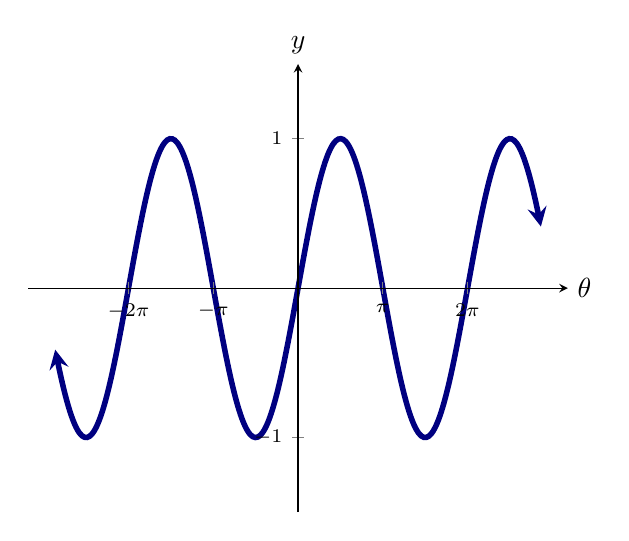
\begin{tikzpicture} 
  \begin{axis}[
            domain=-10:10, ymax=1.5, xmax=10, ymin=-1.5, xmin=-10,
            xtick={-6.28, -3.14, 3.14, 6.28}, 
            xticklabels={$-2\pi$, $-\pi$, $\pi$, $2\pi$},
            axis lines =center,  xlabel={$\theta$}, ylabel=$y$,
            ticklabel style={font=\scriptsize},
            every axis y label/.style={at=(current axis.above origin),anchor=south},
            every axis x label/.style={at=(current axis.right of origin),anchor=west},
            axis on top
          ]
          
            \addplot [line width=2, penColor, smooth,samples=200,domain=(-9:9), <->] {sin(deg(x))};

           

  \end{axis}
\end{tikzpicture}
\end{image}



Let's create a new function called $T$, which is a shifted sine function.

\[  T(t) = \sin(t + \tfrac{\pi}{6})  \]



\begin{image}
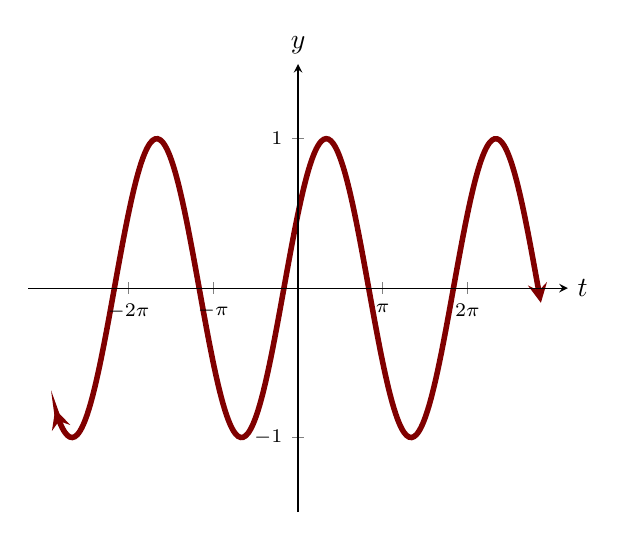
\begin{tikzpicture} 
  \begin{axis}[
            domain=-10:10, ymax=1.5, xmax=10, ymin=-1.5, xmin=-10,
            xtick={-6.28, -3.14, 3.14, 6.28}, 
            xticklabels={$-2\pi$, $-\pi$, $\pi$, $2\pi$},
            axis lines =center,  xlabel={$t$}, ylabel=$y$,
            ticklabel style={font=\scriptsize},
            every axis y label/.style={at=(current axis.above origin),anchor=south},
            every axis x label/.style={at=(current axis.right of origin),anchor=west},
            axis on top
          ]
          
            \addplot [line width=2, penColor2, smooth,samples=200,domain=(-9:9), <->] {sin(deg(x+0.523599))};

           

  \end{axis}
\end{tikzpicture}
\end{image}
This graph looks the same as the one above, except shifted to the left.


$\theta = t + \tfrac{\pi}{6}$   or $\theta - \tfrac{\pi}{6}= t $



Labelling the horizontal axes $\theta$ and $t$ makes it easier to compare.

\end{example}









\begin{image}
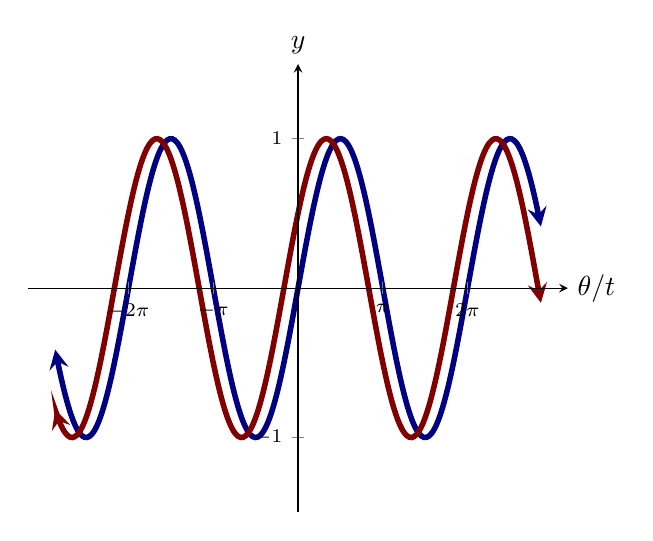
\begin{tikzpicture} 
  \begin{axis}[
            domain=-10:10, ymax=1.5, xmax=10, ymin=-1.5, xmin=-10,
            xtick={-6.28, -3.14, 3.14, 6.28}, 
            xticklabels={$-2\pi$, $-\pi$, $\pi$, $2\pi$},
            axis lines =center,  xlabel={$\theta$/$t$}, ylabel=$y$,
            ticklabel style={font=\scriptsize},
            every axis y label/.style={at=(current axis.above origin),anchor=south},
            every axis x label/.style={at=(current axis.right of origin),anchor=west},
            axis on top
          ]
          
            \addplot [line width=2, penColor, smooth,samples=200,domain=(-9:9), <->] {sin(deg(x))};
            \addplot [line width=2, penColor2, smooth,samples=200,domain=(-9:9), <->] {sin(deg(x+0.523599))};

           

  \end{axis}
\end{tikzpicture}
\end{image}











\begin{example} Sine



Graph of $y = \sin(\theta)$.

\begin{image}
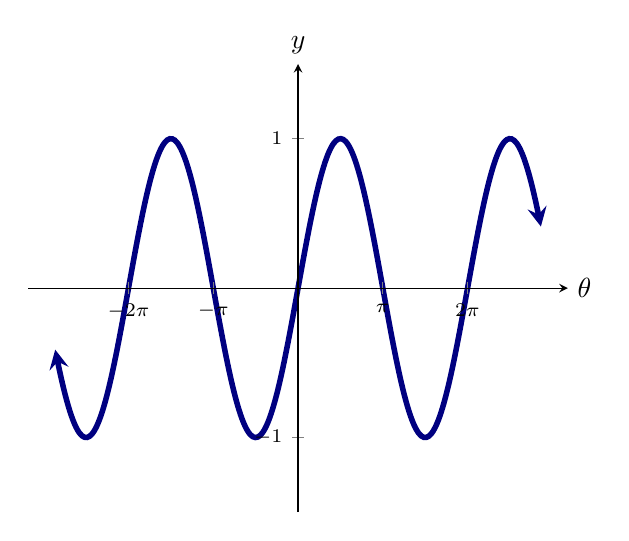
\begin{tikzpicture} 
  \begin{axis}[
            domain=-10:10, ymax=1.5, xmax=10, ymin=-1.5, xmin=-10,
            xtick={-6.28, -3.14, 3.14, 6.28}, 
            xticklabels={$-2\pi$, $-\pi$, $\pi$, $2\pi$},
            axis lines =center,  xlabel={$\theta$}, ylabel=$y$,
            ticklabel style={font=\scriptsize},
            every axis y label/.style={at=(current axis.above origin),anchor=south},
            every axis x label/.style={at=(current axis.right of origin),anchor=west},
            axis on top
          ]
          
            \addplot [line width=2, penColor, smooth,samples=200,domain=(-9:9), <->] {sin(deg(x))};

           

  \end{axis}
\end{tikzpicture}
\end{image}



$\sin(\theta)$ is periodic with a period of $2\pi$.  If it is shifted by $2\pi$ or any integer multiple of $2\pi$, then the resulting function is again $\sin(\theta)$.


\[    \sin(\theta + 2k\pi) = \sin(\theta)   \,   \text{ where }  \,  k \in \textbf{Z}       \]



\begin{itemize}
\item The zeros of $\sin(\theta)$ are all integer multiples of $\pi$.
\item The maximum value is $1$ and it occurs at:  $\left\{     \frac{\pi}{2} + 2k\pi \, | \, k \in \textbf{Z}     \right\} = \left\{     \frac{(4k+1)\pi}{2} \, | \, k \in \textbf{Z}     \right\}$
\item The minimum value is $-1$ and it occurs at:  $\left\{    \frac{3\pi}{2} + 2k\pi \, | \, k \in \textbf{Z}     \right\} = \left\{    \frac{(4k+3)\pi}{2} \, | \, k \in \textbf{Z}     \right\}$
\end{itemize}


If $\sin(\theta)$ is shifted left by $\frac{\pi}{2}$, then we get $\cos(\theta)$.


\[    \sin\left(\theta + \frac{\pi}{2}\right) = \cos(\theta)   \]


Graph of $y = \cos(\theta)$.

\begin{image}
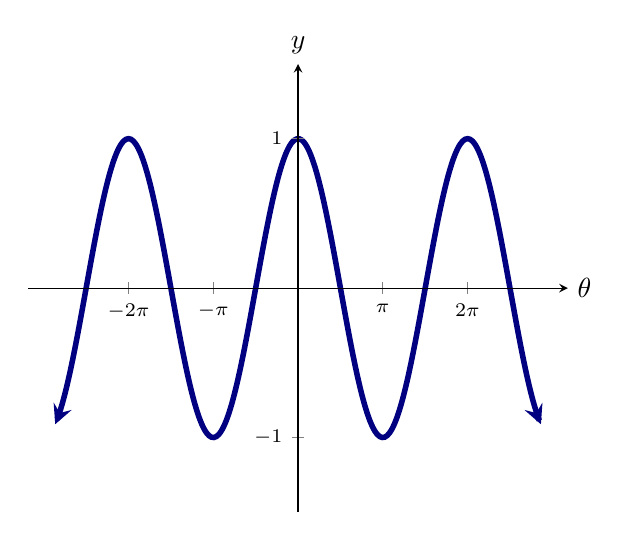
\begin{tikzpicture} 
  \begin{axis}[
            domain=-10:10, ymax=1.5, xmax=10, ymin=-1.5, xmin=-10,
            xtick={-6.28, -3.14, 3.14, 6.28}, 
            xticklabels={$-2\pi$, $-\pi$, $\pi$, $2\pi$},
            axis lines =center,  xlabel={$\theta$}, ylabel=$y$,
            ticklabel style={font=\scriptsize},
            every axis y label/.style={at=(current axis.above origin),anchor=south},
            every axis x label/.style={at=(current axis.right of origin),anchor=west},
            axis on top
          ]
          
            \addplot [line width=2, penColor, smooth,samples=200,domain=(-9:9), <->] {cos(deg(x))};

           

  \end{axis}
\end{tikzpicture}
\end{image}



\end{example}




This agrees with the unit circle.  As you move along the unit circle, the right/vertical coordinate (sine) has the same value as the left/horizontal coordinate (cosine) back a quarter-circle.









\begin{example} Absolute Value



Graph of $y = |x|$.



\begin{image}
\begin{tikzpicture} 
  \begin{axis}[
            domain=-10:10, ymax=10, xmax=10, ymin=-10, xmin=-10,
            axis lines =center, xlabel=$x$, ylabel=$y$,
            ytick={-10,-8,-6,-4,-2,2,4,6,8,10},
            xtick={-10,-8,-6,-4,-2,2,4,6,8,10},
            ticklabel style={font=\scriptsize},
            every axis y label/.style={at=(current axis.above origin),anchor=south},
            every axis x label/.style={at=(current axis.right of origin),anchor=west},
            axis on top
          ]
          
          \addplot [line width=2, penColor, smooth, samples=200, domain=(-7:7),<->] {abs(x)};
        

  \end{axis}
\end{tikzpicture}
\end{image}





What does the graph of $z = |t-2|$ look like?

This is a shift from the basic absolute value graph.  All we really need to know is where is the corner.  

\begin{center}
\textbf{\textcolor{blue!55!black}{The corner occurs when the inside of the absolute value equals $0$.}} 
\end{center}



$t-2=0$ when $t=2$.  That is where the new corner sits.









\begin{image}
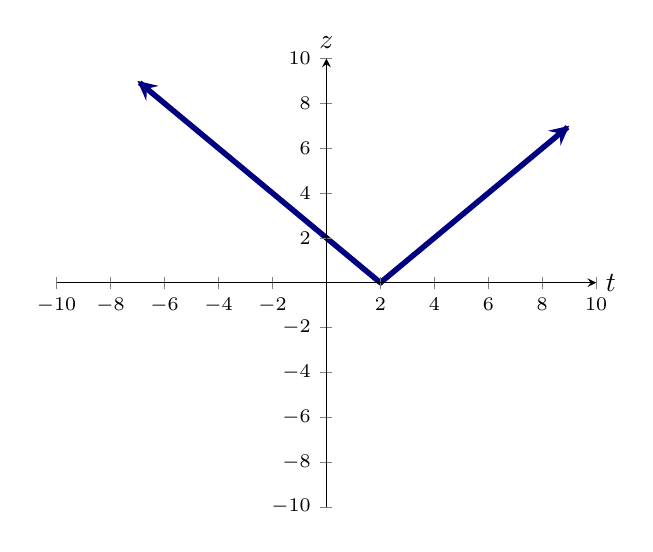
\begin{tikzpicture} 
  \begin{axis}[
            domain=-10:10, ymax=10, xmax=10, ymin=-10, xmin=-10,
            axis lines =center, xlabel=$t$, ylabel=$z$,
            ytick={-10,-8,-6,-4,-2,2,4,6,8,10},
            xtick={-10,-8,-6,-4,-2,2,4,6,8,10},
            ticklabel style={font=\scriptsize},
            every axis y label/.style={at=(current axis.above origin),anchor=south},
            every axis x label/.style={at=(current axis.right of origin),anchor=west},
            axis on top
          ]
          
          \addplot [line width=2, penColor, smooth, samples=200, domain=(-7:9),<->] {abs(x-2)};
        

  \end{axis}
\end{tikzpicture}
\end{image}








\end{example}


Much of graphing follows this example.  \\


There are \textbf{important/strategic points} for the function's graph. You identify the new position of those points.  Then, the shifted graph follows the basic shape of the original graph.






For example, $y = \log_k(t)$ [ including $y = \ln(t)$ ] has a vertical asymptote when the inside of the logarithm equals $0$. The zero, and corresponding horizontal intercept, occurs when the inside equals $1$.  






\begin{example}

Here is the graph of $y = \log_2(t+5)$.

\begin{itemize}
\item vertical asymptote: $t+5=0$, when $t=\answer{-5}$
\item horizontal intercept: $t+5=1$, when $t=\answer{-4}$
\end{itemize}


\begin{image}
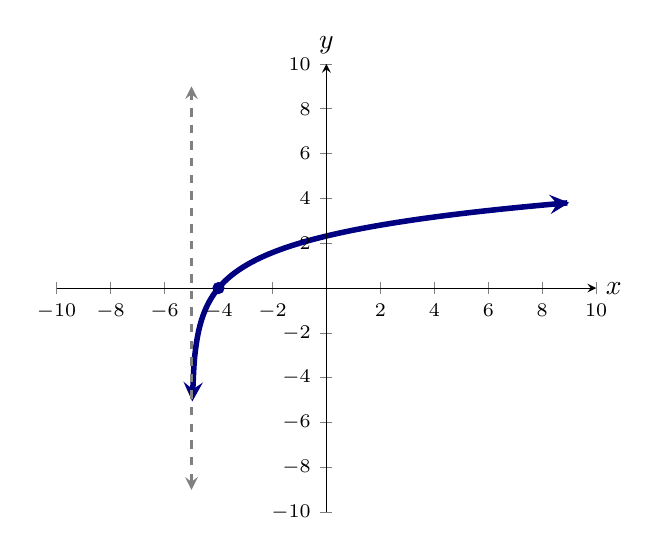
\begin{tikzpicture} 
  \begin{axis}[
            domain=-10:10, ymax=10, xmax=10, ymin=-10, xmin=-10,
            axis lines =center, xlabel=$x$, ylabel=$y$,
            ytick={-10,-8,-6,-4,-2,2,4,6,8,10},
            xtick={-10,-8,-6,-4,-2,2,4,6,8,10},
            ticklabel style={font=\scriptsize},
            every axis y label/.style={at=(current axis.above origin),anchor=south},
            every axis x label/.style={at=(current axis.right of origin),anchor=west},
            axis on top
          ]
          
          \addplot [line width=2, penColor, smooth,samples=200,domain=(-4.97:9),<->] {ln(x+5)/ln(2)};
          \addplot [line width=1, gray, dashed,domain=(-9:9),<->] ({-5},{x});

          \addplot[color=penColor,only marks,mark=*] coordinates{(-4,0)}; 

           

  \end{axis}
\end{tikzpicture}
\end{image}


The graph looks the same as the basic logarithm graph, just slid left $5$.




\end{example}









\begin{example} Shifting Domains


Let $M$ be a function with domain $[-7,-4) \cup [-2,1] \cup [1,7)$. \\

Below is the graph of $y = M(d)$.




\begin{image}
\begin{tikzpicture}
  \begin{axis}[
            domain=-10:10, ymax=10, xmax=10, ymin=-10, xmin=-10,
            axis lines =center, xlabel=$d$, ylabel=$y$,
            ytick={-10,-8,-6,-4,-2,2,4,6,8,10},
            xtick={-10,-8,-6,-4,-2,2,4,6,8,10},
            ticklabel style={font=\scriptsize},
            every axis y label/.style={at=(current axis.above origin),anchor=south},
            every axis x label/.style={at=(current axis.right of origin),anchor=west},
            axis on top
          ]
          
  \addplot [draw=penColor,very thick,smooth,domain=(-7:-4)] {-x-6};
  \addplot [draw=penColor,very thick,smooth,domain=(-2:1)] {-7};
  \addplot [draw=penColor,very thick,smooth,domain=(1:7)] {-x+7};
  
  \addplot[color=penColor,only marks,mark=*] coordinates{(-7,1)}; 
  \addplot[color=penColor,fill=white,only marks,mark=*] coordinates{(-4,-2)}; 
  \addplot[color=penColor,only marks,mark=*] coordinates{(-2,-7)}; 
  \addplot[color=penColor,only marks,mark=*] coordinates{(1,-7)}; 
  \addplot[color=penColor,only marks,mark=*] coordinates{(1,6)}; 
  \addplot[color=penColor,fill=white,only marks,mark=*] coordinates{(7,0)}; 


    \end{axis}
\end{tikzpicture}
\end{image}
A new function is created by shifting $M$. \\





The function $H(k)$ is defined as $H(k) = M(k+3)$ with the induced domain.



\begin{question}

We can see that $M(-7) = 1$.  This tells us that $H\left(\answer{-10}\right) = \answer{1}$. \\

There is an open dot on the graph of $y= M(d)$  when $d = -4$.  There will be a corresponding open dot on the graph of $z = H(k)$ when $k = \answer{-7}$.

\end{question}


\begin{question}

There is a horizontal line segment in the graph of $y = M(d)$ from $(-2, -7)$ to $(1, -7)$.  There will be a horizontal line segment in the graph of $z = H(k)$ from $\left(\answer{-5}, -7\right)$ to $\left(\answer{-2}, -7\right)$.

\end{question}



\begin{question}

There is a closed dot on the graph of $y= M(d)$  when $d = 1$.  There will be a corresponding closed dot on the graph of $z = H(k)$ when $k = \answer{-2}$. \\


There is an open dot on the graph of $y= M(d)$  when $d = 7$.  There will be a corresponding open dot on the graph of $z = H(k)$ when $k = \answer{4}$.

\end{question}




\end{example}













































\begin{center}
\textbf{\textcolor{green!50!black}{oooo-=-=-=-ooOoo-=-=-=-ooooo}} \\

more examples can be found by following this link\\ \link[More Examples of Shifting]{https://ximera.osu.edu/csccmathematics/precalculus/precalculus/transformations/examples/exampleList}

\end{center}




\end{document}
